\chapter{Softwareimplementierung}
\label{software}
\section{Softwareanforderung}
Ein weiterer Teil des Projektes ist die Softwareimplementierung. Die Aufgabe dieser erstreckt sich von der Bildverarbeitung über den Objekterkennungsprozess bis hin zu der Regelung und Steuerung der Drohne. Dabei muss sie verschiedensten Kriterien genügen.\\
\\
Da sie Signale von einem Externen Bauteilen wie dem PX4 oder dem Abstandssensor über das Interface ROS (siehe Kapitel \ref{gesamtintegration}) kann es zu Datenverlust kommen. Bedingt durch die unterschiedlichen Taktrate der Prozessoren. Deshalb muss auch bei gelegentlich fehlenden Datenpaketen der Rest verarbeitet und die Drohne auf Grundlage dieser geregelt werden.\\
\\
Der PX4-Controller schreibt eine Datenrate von 20 Hz vor. Also muss in dieser Datenrate die Sollposition der Drohne geschickt werden. Fallen diese aus, so geht die Drohne in den Offboard-Modus und steigt auf 10 m Höhe, um dann automatisch zur Startposition zurückzukehren. Dies wäre bei einer Raumhöhe von 2,5 m fatal. Leider kann man diese „Schutzfunktion“ nicht abschalten da sie fest im Betriebssystem des PX4-Controllers verankert ist. Demzufolge darf das Signal der Position nie ausbleiben.\\
\\
Um dies zu erreichen, darf sich die Regeleinheit der Drohne nie aufhängen. Alle Schleifen müssen deshalb ein zeitliches Abbruchsignal haben, um eine Auslastung des Arbeitsspeichers zu verhindern. Aufgrund des Gewichtes muss ein leichter Controller gewählt werden(siehe Hardware Komponenten). Da wir aufgrund der Software Inkompatibilität des Pi-4 mit dem PX4-Controller einen Pi-3 gewählt haben steht ein maximaler Arbeitsspeicher von 1 Gb zur Verfügung. Dabei hat er 2 Kerne und kann somit effektiv 2 Aufgaben gleichzeitig ausführen. Die Software muss also sehr ressourcensparend geschrieben sein.\\
\\
Aufgrund der Struktur von ROS empfiehlt es sich, einen Event basierten Programmablauf zu schreiben. Dabei löst ein Event, also eine Aktion die stattfindet, einen Programmablauf aus. In diesem Fall sind die Events eingehende Datenpakete für die entsprechende Node (Siehe Programmstruktur). Diese werden verarbeitet. Dadurch kann sichergestellt werden, dass jedes Datenpaket verarbeitet wird, unabhängig in welchem Abstand es ankommt. Durch diese Warte-Bedien-Struktur wird eine maximale Effizienz erreicht, da das Programm keine Schritte doppelt auf nicht aktualisierte Werte anwendet und so Prozessorzeit spart.
\section{Python als Programmiersprache}
Wie es häufig in der Entwicklung der Fall ist, stehen auch hier für die Implementierung
der Software auf dem RPi verschiedene Plattformen, Frameworks und
Programmiersprachen zu Verfügung. Bei der Wahl der Programmiersprache ist zu beachten das sie möglichst einfach und bereits relativ alt ist. Der Vorteil von alten Programmiersprachen ist, dass es eine umfangreiche Beispielsammlung gibt. Dadurch kann man sich leicht an bereits vorhandenem Code orientieren.
Anforderungs-bedingt muss die Programmiersprache möglichst ressourcenschonend sein.
Dadurch fallen alle grafischen Programmiersprachen wie Matlab, Simulink, Labview etc. heraus. Diese haben aufgrund ihres unstrukturierten Programmablaufs, eine eher schlechte Laufzeit.\\ 

Eine der am weitesten verbreiteten Programmiersprachen ist Java. Der Vorteil von Java ist, dass es plattformübergreifend funktioniert. Leider verwendet Java dafür eine Virtuelle Java Maschine. Also ein Betriebssystem, dass noch mal über dem Betriebssystem liegt. Dies verringert die Laufzeit von Java enorm. Ein weiteres Problem liegt darin, dass Schnittstellen immer plattformabhängig sind(USB, D-Sub, Ethernet etc.). Dadurch werden sie durch Java nur schlecht unterstützt. Aus diesen Gründen konnte Java ebenfalls nicht gewählt werden.\\

Eine weitere Alternative ist eine C-Programmiersprache(C++, C etc.). Diese haben den großen Vorteil, dass sie echtzeitfähig sind. Sie können also unter Umständen garantieren, dass das Ergebnis des Algorithmus nach einer bestimmten Zeit feststeht. Dies ist für eine Drohnensteuerung sehr geeignet, da man garantieren sollte, dass sie Drohne in einem bestimmten Zeitintervall überwacht wird. Außerdem sind C-Sprachen sehr Hardware nah geschrieben, wodurch die Laufzeit sehr gut ist. Allerdings wird die Hought-Transformation der Bibliothek Open-CV genutzt. Diese Bibliothek ist allerdings nicht echtzeitfähig, wodurch der große Vorteil von C verloren geht. Des Weiteren ist es sehr schwer/mühselig Open-CV in C zu implementieren.\\

Außerdem ist Python eine Alternative. Python ist leider nicht echtzeitfähig. Jedoch ist es sehr benutzerfreundlich, hinsichtlich des Importierens von Bibliotheken. Es ist nicht so hardwarenah wie C, allerdings immer noch deutlich näher als Java oder Labview. Außerdem gibt es zahlreiche Beispiele für Python und das Ansteuern von Schnittstellen geht problemlos. Aus all diesen Gründen ist die Wahl auf Python gefallen.

\section{Vergleich Monolithische Single Application und Service Oriented Architecture}
\subsection{Monolithische Single Application}
Bei der Softwarearchitektur wurde sich zunächst an einer normalen objektorientierten Struktur bedient: Es gibt eine main-Datei, welche vergleichsweise
klein ist und nur die grobe Struktur bzw. den Gesamtablauf darstellt. Diese ruft dann weitere Softwaremodule auf, die die Unteraufgaben, wie beispielsweise das Empfangen und Verarbeiten von Bilddaten, implementiert. Ein Problem, das hier recht schnell auftritt ist, dass theoretisch zwei Prozesse gleichzeitig ablaufen müssen. Wenn ein Motormodul beispielsweise gerade darauf wartet, dass die Sollposition erreicht wurde, müsste in einem Programmierstrang, in dem ein Befehl nach dem anderen ausgeführt wird, das Kameramodul mit der Verarbeitung des Bildes auf das Motormodul warten, obwohl das Motormodul gerade gar nichts tut, außer auf den
Motor in der echten Welt zu warten, bis er die gewünschte Position hat. Da das Kameramodul aber an das Motormodul eventuell kommunizieren muss, dass das
Paket gar nicht mehr an der richtigen Stelle ist, weil der Quadrokopter aufgrund äußerer Umstände nicht ganz stillsteht, müssen beide Module gleichzeitig arbeiten und
miteinander kommunizieren können. \\

In der traditionellen Softwareentwicklung gibt es dafür sogenannte Threads. Diese sind separate Ausführungsstränge, die quasi gleichzeitig ausgeführt werden und sich dann beispielsweise ein Datenobjekt im Speicher teilen und über dieses miteinander kommunizieren können. Das entspricht dann einer Dreischicht-Architektur (siehe Abb. \ref{fig:Dreischichtarchitektur}).

Wichtig bei dieser Art der Architektur ist, dass jede Schicht nur auf die nächst untere zugreifen darf, um einen reibungslosen Ablauf garantieren zu können. In diesem Fall greifen nun die Threads $T_1$, $T_2$ ... $T_n$ nicht direkt auf den Speicher zu, sondern müssen den Weg über die Datenzugriffsschicht gehen. Diese stellt unter anderem mittels Semaphoren sicher, dass immer nur ein Thread auf die entsprechende Ressource zugreifen kann. Damit wird verhindert, dass beispielsweise $T_1$ schreiben und $T_2$ gleichzeitig lesen möchte. Dies würde zu einem Speicherkonflikt führen und das Programm wird abstürzen. \cite{riedel2019itarch}

\begin{figure}[h]
	\centering
	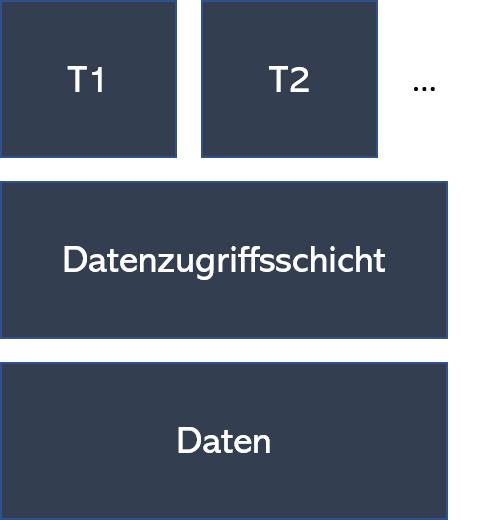
\includegraphics[scale=0.5]{"Grafiken/dreischichtarchitektur.png"}
	\caption{Dreischichtarchitektur}
	\label{fig:Dreischichtarchitektur}
\end{figure}



\subsection{Service Oriented Architecture}
Bis zu einem gewissen Grad war es möglich die geforderten Funktionalitäten mit Multithreading zu implementieren. Allerdings wurde es im Laufe der Entwicklung immer komplizierter, da Bilddaten beispielsweise von zwei Ressourcen abhängen, die nicht immer verfügbar sind: zum einen der Speicherplatz im Datenobjekt, das andere Threads lesen und damit belegen wollen und zum anderen von der Kamera selbst, die natürlich auch nicht willkürlich Bilddaten liefert. Das zu synchronisieren ist zwar theoretisch möglich, praktisch aber mit einer Menge schwer wartbarem Code verbunden, der das Problem unnötig kompliziert löst.
\subsection{Robot Operating System}
Deshalb basiert die endgültige Software auf ROS, das genau diese Probleme adressiert. ROS steht dabei für Robot Operating System und ist ein Framework, das auf dem Publisher-Subscriber-Modell (P/S-Modell) basiert. Die Idee ist dabei, dass es verschiedene Themen (Topics) gibt, in die verschiedene dezentrale Skripte, die gleichzeitig laufen, Informationen zu einzelnen Themen veröffentlichen oder abonnieren können. So gibt es beispielsweise ein Kameraskript, das das Bild und die erkannte Position des Pakets veröffentlicht und ein Motorskript abonniert die Paketposition und kann daraus dann weitere Schlüsse ziehen. Ein anderes Skript könnte dann auf einem anderen Rechner (z.B. Laptop) im gleichen (WLAN-) Netzwerk das Kamerabild abbonnieren und mit sehr wenig Programmieraufwand anzeigen. Das elegante dabei ist, dass sämtliche vorher beschriebene Multithreading-Probleme dabei vom sogenannten ROS-Core, der zentrale Schaltstelle des ROS, übernommen werden und damit die einzelnen (selbstgeschriebenen) Skripte sehr entschlackt werden. Das macht es deutlich einfacher diese zu debuggen. ROS ist zudem sehr gut dokumentiert und für viele Probleme gibt es bereits vorgefertigte Skripte, die Dank des einfachen P/S-Modells auch einfach anzubinden sind.
\subsection{ROS als Beispiel einer Service Oriented Architecture (SOA) / Microservices}
Die Architektur hinter ROS ist dabei keine neue Erfindungen, sondern basiert im Gegensatz zum Ansatz der Schichtenarchitektur auf dem Prinzip der serviceorientierten Architektur (SOA). 

Bei der SOA spielt der (Enterprise) Service Bus eine zentrale Rolle. Er ist das Bindeglied zwischen allen anderen Knotenpunkten im Netzwerk und stellt sicher, dass die Kommunikation funktioniert. Bei ROS ist das der ROS-Master, der über den Befehl 
\begin{lstlisting}[language=bash]
$ roscore
\end{lstlisting}
gestartet werden kann. Über ihn kommunizieren die Knoten miteinander, wobei jeder Knoten eine logisch abgeschlossene Aufgabe übernimmt und von außen über eine API angesprochen werden kann. Im Fall des Quadrokopters existiert nun beispielsweise ein Knoten, der das Kamerabild publiziert, einer, der das Bild verarbeitet und einer, der die Steuerung auf Basis der Bilddaten durchführt. Durch diese Modularität gibt es einige Vorteile. So ist es damit sehr leicht einen Knoten auszutauschen, zu erweitern oder neue Knoten hinzuzufügen. Zudem ist das System deutlich stabiler als eine monolithische Lösung, da bei einem fehlerhaften Knoten nur die Knoten ausfallen, die von diesem Ausfall logisch betroffen sind. Alle unabhängigen Knoten werden weiterhin funktionieren. Bei einer monolithischen Lösung führt ein Modulausfall zum Ausfall des Gesamtsystems. 

Aber einer gewissen Granularität spricht man von Microservices. Diese folgen der Strategie 
``Erledige nur eine Aufgabe und erledige sie gut'' %ToDo:\cite{riedel:it-arch}
Bei ``normalen'' SOAs sind die Knoten tendenziell groß und implementieren viele Funktionalitäten auf einmal. Microservices hingegen sind sehr klein und erledigen nur eine bestimmte Aufgabe. In der finalen Gesamtarchitektur kommen Knoten zum Einsatz, die sowohl den normalen SOAs als auch den Microservices zugewiesen werden können.

\begin{figure}[h]
	\centering
	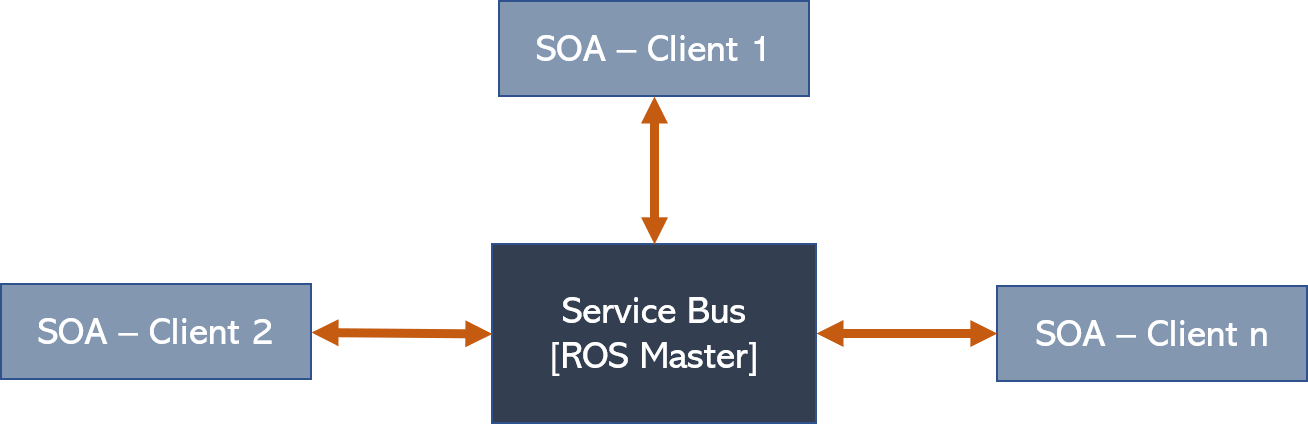
\includegraphics[scale=0.5]{"Grafiken/soa.png"}
	\caption{Service Oriented Architecture}
	\label{fig:meine-grafik}
\end{figure}

\section{Finale Gesamtarchitektur - Übersicht}
In der finalen Gesamtarchitektur (siehe Abb. \ref{fig:gesamtarch}) gibt es insgesamt drei ROS Instanzen: Die erste läuft auf dem Quadrokopter selber und dient als Schnittstelle zur Firmware des Quadrokopters. Der dazugehörige Knoten heißt Mavros, welcher mit MAVLink (Micro Air Vehicle Link) kommuniziert, das die gesamte tatsächliche Steuerung des Quadrokopters übernimmt. Dabei hat der ROS-Core jedoch keine Master-Funktion, sondern verbindet sich über eine serielle Schnittstelle mit dem ROS-Core auf dem RaspberryPi, auf dem der tatsächliche Master-ROS-Core läuft. Dieser ist in einem WLAN-Netzwerk mit einem Laptop, der für Debugging-Zwecke und zum Konfigurieren und Kontrollieren der Bildverarbeitung benötigt wird. Auch auf dem Laptop läuft ein ROS-Core, wobei auch dieser sich mit dem Master auf dem Raspberry Pi verbindet. Im folgenden werden nun die einzelnen Knoten genauer vorgestellt.

\begin{figure}[h]
	\centering
	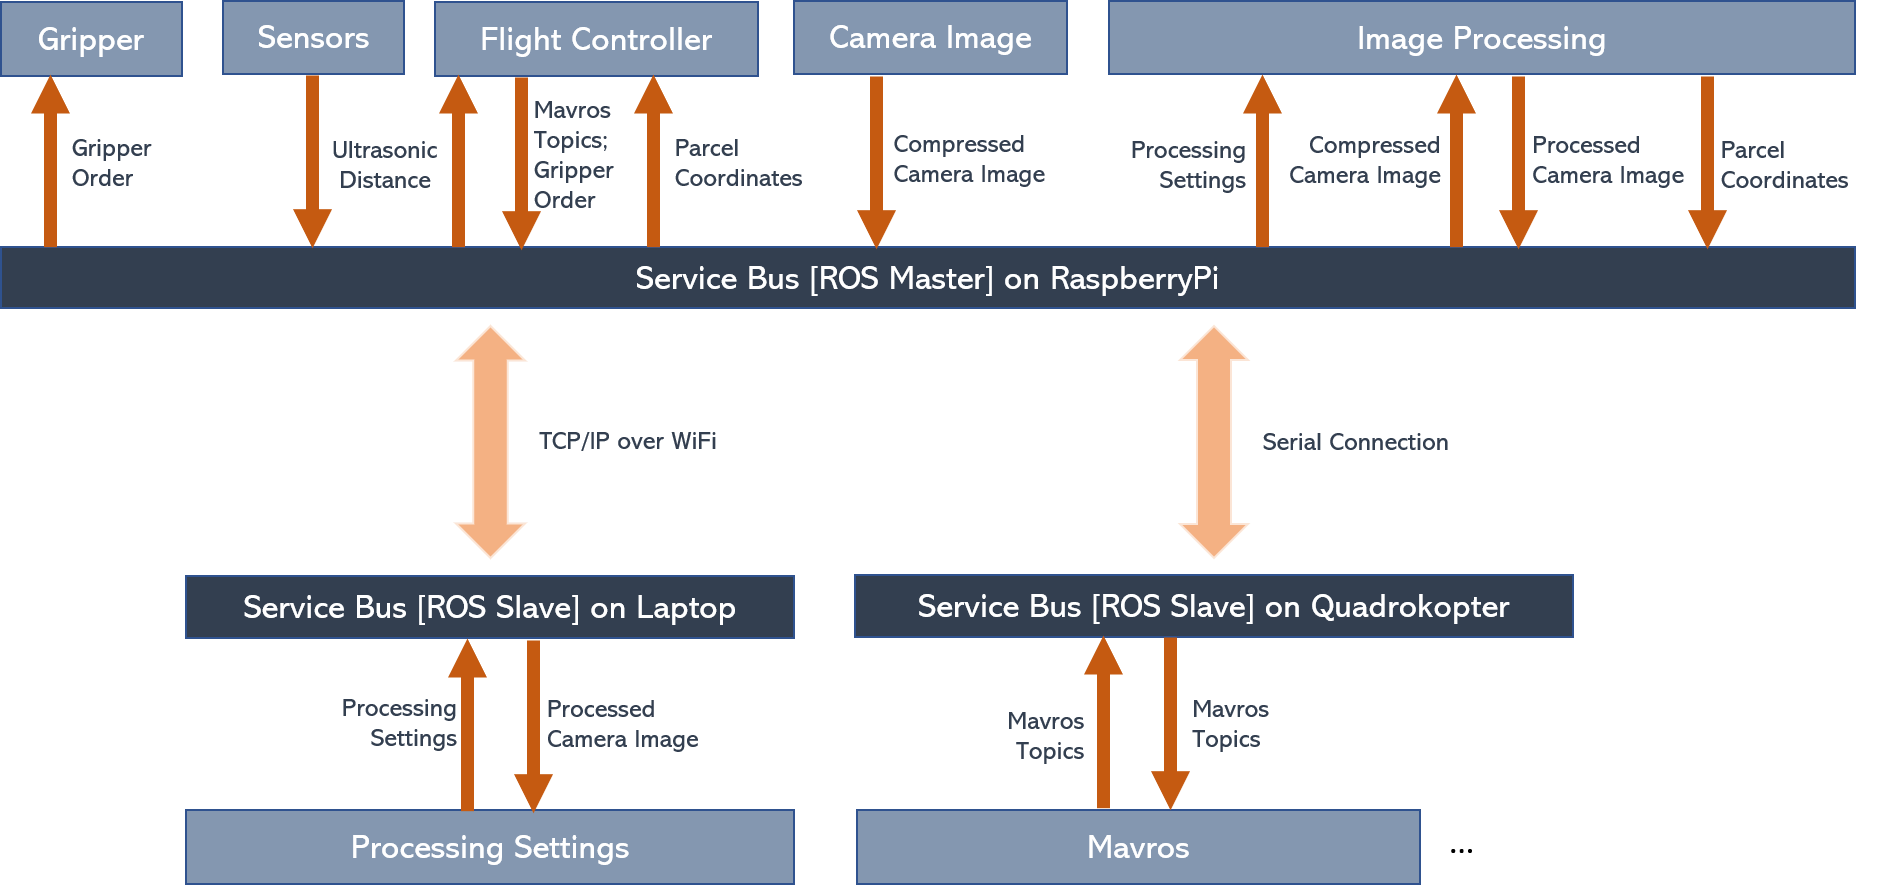
\includegraphics[scale=0.41]{"Grafiken/gesamtarchitektur.png"}
	\caption{Service Oriented Architecture}
	\label{fig:gesamtarch}
\end{figure}

\subsection{Camera Image} ``Camera Image'' ist ein einfacher Publisher, der das Bild der Dronenkamera komprimiert und über den Service Bus den anderen Knoten im Netzwerk als serialisiertes numpy-Array zu Verfügung stellt. Aufgrund der später folgenden rechenintensiven Bildverarbeitung sendet dieser in der finalen Version das Bild jedoch nur mit 10 Hz. Dies is jedoch immer noch ausreichend, da sich die Geschwindigkeit der Drone nicht schnell ändern wird. 
\subsection{Image Processing} ``Image Processing'' empfängt die Bilddaten von Camera Image und wir zudem über das Topic Processing-Settings vom Laptop aus konfiguriert. Dieser Knoten filtert dann das Bild um anschließend die Position und Drehung des Pakets zu ermitteln. Das gefilterte Bild und die Koordinaten als Typ
\begin{lstlisting}[language=Python]
PoseStamped
\end{lstlisting}
des Pakets werden publiziert. Dieser Nachrichtentyp enthält unter 
\begin{lstlisting}[language=Python]
geometry_msgs/Point
\end{lstlisting}
drei Koordinaten ($x$, $y$, $z$) wobei in diesem Fall $x$ und $y$ die Position und $z$ die Drehung um die $z$-Achse angibt.

\subsection{Sensors} ``Sensors'' verwaltet alle Sensordaten. In der aktuellen Version ist das jedoch nur der Ultraschallsensor. Die Daten werden gesammelt, aufbereitet, validiert und publiziert. So werden dann beispielsweise die Ultraschalldaten unter der Topic 
\begin{lstlisting}[language=Python]
/sensor_dist
\end{lstlisting}
im Datenformat Float32 mit einer Frequenz von 20 Hz veröffentlicht.

\subsection{Flight Controller} ``Flight Controller'' ist die zentrale Steuereinheit der neuen Funktionalität. Er empfängt alle aufbereiteten Sensordaten wie die Koordinaten des Pakets, Ultraschalldistanz, Sensordaten der Drone etc. und führt die Suche und Anflug des Pakets durch. Er gibt die Flugsteuerbefehle an Mavros über die serielle Schnittstelle weiter und gibt Greifbefehle weiter. Mehr dazu ist im Kapitel \ref{gesamtintegration} zu finden. 

\subsection{Datenübertragungsformate}
Es war sehr schwierig, die richtigen Formate zu wählen da Python im Allgemeinen eher unsauber mit den verschiedenen Datentypen umgeht. So gibt es z. B. keinen Unterschied zwischen einem 32-Bit oder einem 64-Bit Integrer. Falls die Zahl außerhalb des darstellbaren Bereiches des 32-Bit Interger liegt, so erweitert der Python-Interpreter es selbstständig zu einem 64 Bit Integer. ROS ist hingegen sehr typenspezifisch, wodurch es zuerst einige Unklarheiten bezüglich der Typen gab und diese dementsprechend verändert werden mussten.\\


\section{Implementierung der Kommunikation in ROS}
Wie bereits erwähnt basiert ROS auf dem Publisher/Subscriber Prinzip. Ein Knoten kann in ROS sowohl Publisher als auch Subscriber sein und das auch für mehrere Topics. Die Topics sind dabei hierarchisch aufgebaut und gehen vom Groben ins Feine. So publiziert beispielsweise der ``Camera Image'' Knoten das komprimierte Bild in 

\begin{lstlisting}[language=Python]
/camera/image/compressed
\end{lstlisting}. 

Anhand dieses Beispiels soll nun dargelegt werden, wie man prinzipiell bei der Erstellung eines Nodes vorgeht.


\subsection{Kamera Publisher}
Zunächst muss eine Datei mit dem Namen des Knotens und der Endung ``.py'' im entsprechenden Paketordner im src-Ordner des Catkin-Workspaces erstellt werden. Diese kann dann in PyCharm geöffnet werden, wenn nicht schon das gesamte Paket als Projekt geöffnet wurde.
Um klarzumachen, dass es sich hierbei um ein Python File handelt, muss die Datei mit 


\begin{lstlisting}[language=Python]
#!/usr/bin/env python3
\end{lstlisting}

starten, um die Pythonumgebung auszuwählen. Es folgt nun für gewöhnlich die Lizenzerklärung zur Datei. Es sollten nun 

\begin{lstlisting}[language=Python]
numpy, time, cv2, roslib, rospy
\end{lstlisting}

importiert werden. ``numpy'' ist eine Bibliothek zum effizienten Arbeiten mit numerischen Arrays. ``time'' gibt Zugriff auf die aktuelle Systemzeit. ``cv2'' ist die Python-Version von OpenCV, mit der die Bildverarbeitung implementiert wird. ``roslib'' und ``rospy'' sind die Schnittstellen zum ROS-Bus. Außerdem muss für dieses Skript

\begin{lstlisting}[language=Python]
CompressedImage
\end{lstlisting}aus der ROS-Bibliothek 

\begin{lstlisting}[language=Python]
sensor_msgs.msg
\end{lstlisting} importiert werden. 

Es empfiehlt sich nun die gesamte Funktionalität mittels 

\begin{lstlisting}[language=Python]
def function_name
\end{lstlisting}

in eine Funktion zu packen. Dort muss dann zunächst mit 

\begin{lstlisting}[language=Python]
pub = rospy.Publisher("", DataType)
\end{lstlisting}

ein Objekt erstellt werden, wobei hier das Topic 

\begin{lstlisting}[language=Python]
"/camera/image/compressed"
\end{lstlisting}, 

sowie der Datentyp 

\begin{lstlisting}[language=Python]
CompressedImage
\end{lstlisting} 

dem Konstruktor übergeben werden müssen. Mit 

\begin{lstlisting}[language=Python]
rospy.init_node('node_name', 
	anonymous=True)
\end{lstlisting}

registriert sich der Knoten nun am ROS-Service-Bus. Nun wird die Computerbildverarbeitungsbibliothek OpenCV genutzt, um mit 

\begin{lstlisting}[language=Python]
cap = cv2.VideoCapture(0)
\end{lstlisting}

ein Objekt zu erstellen, dass auf den Datenstrom der ersten angeschlossenen Kamera zugreift. Der nun folgende Code soll so lange ausgeführt werden, wie ROS aktiv ist. Dies lässt sich mit 

\begin{lstlisting}[language=Python]
while not rospy.is_shutdown():
\end{lstlisting}

implementieren. Mit 

\begin{lstlisting}[language=Python]
ret, frame = cap.read()
\end{lstlisting}

wird nun der Datenstrom der Kamera ausgelesen und das aktuelle Bild in die Variable 

\begin{lstlisting}[language=Python]
frame
\end{lstlisting}

geschrieben. Jetzt muss mit 

\begin{lstlisting}[language=Python]
msg = CompressedImage()
\end{lstlisting}

ein Nachrichtenpaket des Typs 

\begin{lstlisting}[language=Python]
CompressedImage
\end{lstlisting}

erstellt werden, das mit 

\begin{lstlisting}[language=Python]
msg.header.stamp = rospy.Time.now()
\end{lstlisting}

um einen Zeitstempel erweitert wird und mit 

\begin{lstlisting}[language=Python]
msg.format = "jpeg"
\end{lstlisting}

das richtige Dateiformat erhält. Die Daten des Pakets werden mit der Property 

\begin{lstlisting}[language=Python]
msg.data
\end{lstlisting}

gesetzt. Diese müssen nun aus dem vorher gelesenen 

\begin{lstlisting}[language=Python]
frame
\end{lstlisting}

erstellt werden. Dafür wird zunächst mit 

\begin{lstlisting}[language=Python]
cv2.imencode('.jpg', frame)[1]
\end{lstlisting}

das 

\begin{lstlisting}[language=Python]
frame
\end{lstlisting}

mithilfe von OpenCV in ein JPEG umgewandelt und wird dann mit 

\begin{lstlisting}[language=Python]
np.array()
\end{lstlisting}

zu einem Bildarray transformiert wird und mit

\begin{lstlisting}[language=Python]
tostring()
\end{lstlisting}

serialisiert wird. Nun ist Paket bereit mit 

\begin{lstlisting}[language=Python]
pub.publish(msg)
\end{lstlisting}

an den Service Bus gesendet zu werden. Die Funktion sollte nun mit 

\begin{lstlisting}[language=Python]
if __name__ == '__main__': function_name()
\end{lstlisting}

aufgerufen werden, wobei es Sinn macht den Funktionsaufruf mit einer Ausnahmeregelung für die 

\begin{lstlisting}[language=Python]
rospy.ROSInterruptException
\end{lstlisting}

zu erweitern. 


\subsection{Kamera Subscriber}
Der dazugehörige Subscriber ist im Knoten ``Image Processing'' implementiert und ist dem Publisher gegenüber recht ähnlich aufgebaut. Hier wird jedoch ein Subscriber-Objekt mit 

\begin{lstlisting}[language=Python]
rospy.Subscriber("topic", 
	DataType,
	callback)
\end{lstlisting}

erstellt, wobei callback die Callback-Funktion ist, die aufgerufen wird, wenn eine neue Nachricht in der Topic ankommt. In den Argumenten dieser Funktion eine Variable 

\begin{lstlisting}[language=Python]
msg
\end{lstlisting}

definiert sein, in der die Nachricht bei Empfang gespeichert wird. Der Inhalt der Nachricht kann mit 

\begin{lstlisting}[language=Python]
msg.data
\end{lstlisting}

aufgerufen werden und mit 

\begin{lstlisting}[language=Python]
np.fromstring(data, np.uint8)
\end{lstlisting}

zuerst zu einem 

\begin{lstlisting}[language=Python]
numpy
\end{lstlisting}-Array deserialisiert und dann mit 

\begin{lstlisting}[language=Python]
cv2.imdecode(np_arr, cv2.IMREAD_COLOR)
\end{lstlisting}

zu einem für OpenCV verarbeitbarem Format dekodiert werden. Der darauf folgende Code zur Bildverarbeitung ist in Kapitel \ref{bilderkennung}. beschrieben. 

\section{Starten und Automation eines ROS-Systems}
Damit die Knoten auch lauffähig sind, müssen die Dateien zunächst mit 

\begin{lstlisting}[language=bash]
chmod +x
\end{lstlisting}

für den Kernel ausführbar gekennzeichnet werden. Nun können, nachdem 

\begin{lstlisting}[language=bash]
roscore
\end{lstlisting}

ausgeführt wurde, in einem jeweils neuen Terminaltab mit 

\begin{lstlisting}[language=bash]
rosrun paketname knotenname.py
\end{lstlisting}

die verschiedenen Knoten ausgeführt werden. Mit 

\begin{lstlisting}[language=bash]
rostopic echo /topic/name
\end{lstlisting}

können die Nachrichten der verschiedenen Topics überwacht werden. Um das alle nicht jedes Mal von Hand machen zu müssen, gibt es bei ROS sogenannte Launch-Files, die, wenn ausgeführt, nicht nur einen ROS-Core ausführen, sondern auch alle notwendigen Knoten startet, Umgebungsvariablen setzt etc. Das Launch File basiert auf XML und enthält innerhalb des 

\begin{lstlisting}[language=xml]
<launch></launch>
\end{lstlisting}Tags alle Komponenten. Ein Knoten ist dabei recht selbsterklärend aufgebaut: 

\begin{lstlisting}[language=xml]
<node name="CameraImagePub" 
	pkg="parcelcopter" 
	type="CameraImagePub.py"/>\end{lstlisting}

Innerhalb des Tags können außerdem Startparameter mit 

\begin{lstlisting}[language=bash]
arg
\end{lstlisting}

definiert werden. Mit dem ``env''-Tag können zudem Umgebungsvariablen gesetzt werden.

Man bemerke hier die Modularität und Stabilität von ROS. Denn die Knoten geben keinen Fehler aus, obwohl ein anderer Knoten, der eigentlich für die Ausführung von Nöten ist, noch gar nicht gestartet ist. Sobald dieser bereit ist, fangen die davon abhängigen Knoten automatisch an zu arbeiten. 

\section{Mavros und Simulation}
Die Simulation der Drohne erfolgt in Gazebo. Dafür wird ein PX4-Controller simuliert. Gazebo greift die Signale von dem ROS Interface ab und verarbeitet sie. Dafür wird eine FPL-Drohne simuliert. Ihre Daten sendet dann Gazebo wieder an den PX4-Controller. Weiterhin sendet es einen Video-Stream mit den simulierten Bildern. Dieser wird dann von der Node ImagePub erkannt und in ROS gestreamt. Eigentlich kommt er schon über ROS aber auf diesem Wege ist es realitätsgetreuer. (Die Alternative wäre einfach eine andere Quelle für den ImagePub anzugeben.) Auf diesem Wege kann die Drohne nahezu eins zu eins simuliert werden. \\
\\
Auf diesem Wege wurden bereits viele Fehler wie z. B. Vorzeichenfehler bei den Berechnungen gefunden. Jedoch ist es etwas kompliziert neue Drohnen zu implementieren, da dies erst die Umgebung programmiert werden muss. Unten sieht man einen Kurzfilm, welcher eine Simulation zeigt.


Auch bei der Simulation ist ROS von Vorteil, da man im Testmodus einfach einen Sensor simulieren kann ohne die eigentlichen funktionsverarbeitenden Programme umschreiben zu müssen. Diese Programme laufen dann auf einem externen PC, der sich im gleichen Netzwerk wie die der Pi befindet, und senden regelmäßig ``Fake'' Nachrichten (auch als Fake News) bekannt.
Außerdem kann man so über einen externen PC einfach den Datenfluss kontrollieren, da man quasi die Rohdaten abrufen kann, um die Funktion der einzelnen Programme zu überprüfen. Das ist natürlich auch ein gewisses Sicherheitsrisiko, weshalb die eingehende Kommunikation in den Service Bus beispielsweise durch ein sicheres WiFi-Netzwerk restriktiert werden muss. 
